\chapter{Basics} \label{sec:basics}
In this chapter, the necessary fundamentals are established in order to provide the basis for the following chapters.  
First, Chapter \ref{sec:used_hardware} describes and justifies the hardware used in this work.  
Subsequently, Chapters \ref{subsec:yocto} and \ref{subsec:linux_stack} introduce the basics of Yocto Linux and explain how \ac{WLAN} is implemented in Linux.  
Chapters \ref{subsec:qos} through \ref{subsec:mac} then cover \ac{QoS}, the characteristics of Wi-Fi 4 to 7 and the different types and functionalities of \ac{MAC}.  
Finally, the fundamentals of real-time are presented in Chapter \ref{sec:real_time}.  
As mentioned above, the next section focuses on the selected hardware.  

\section{Used Hardware} \label{sec:used_hardware}
First, the requirements for the hardware, particularly for the Wi-Fi cards, are discussed in order to provide the basis for the subsequent explanation of the hardware selection.  
The requirements apply especially to the Wi-Fi card.  
As mentioned in Chapter \ref{subsec:objective}, the Wi-Fi standards 4 through 6e and the frequency bands from 2.4 GHz to 6 GHz are relevant for the tests.  
Therefore, the Wi-Fi card must at least support Wi-Fi 6e.  
In addition, the drivers and firmware of the card should be open, as this ensures greater transparency for time analysis and allows for modifications to investigate their influence.  
Moreover, different Wi-Fi cards with different drivers and firmware are required.  
This makes it possible to compare the impact of components that cannot be replaced or are largely vendor-dependent.  
For the underlying computing unit, compatibility with the Wi-Fi card and affordability are the most relevant criteria.  
Specialized real-time hardware is deliberately avoided, since \ac{WLAN} is not a real-time standard and is more commonly used in mixed systems\footnote{In this context, mixed systems refer to systems that include both real-time and non-real-time requirements or processes. In other words, a system that is not purely designed for real-time but still needs to fulfill such properties, albeit to a lesser extent.}.  

\begin{figure}[ht]
    \centering
    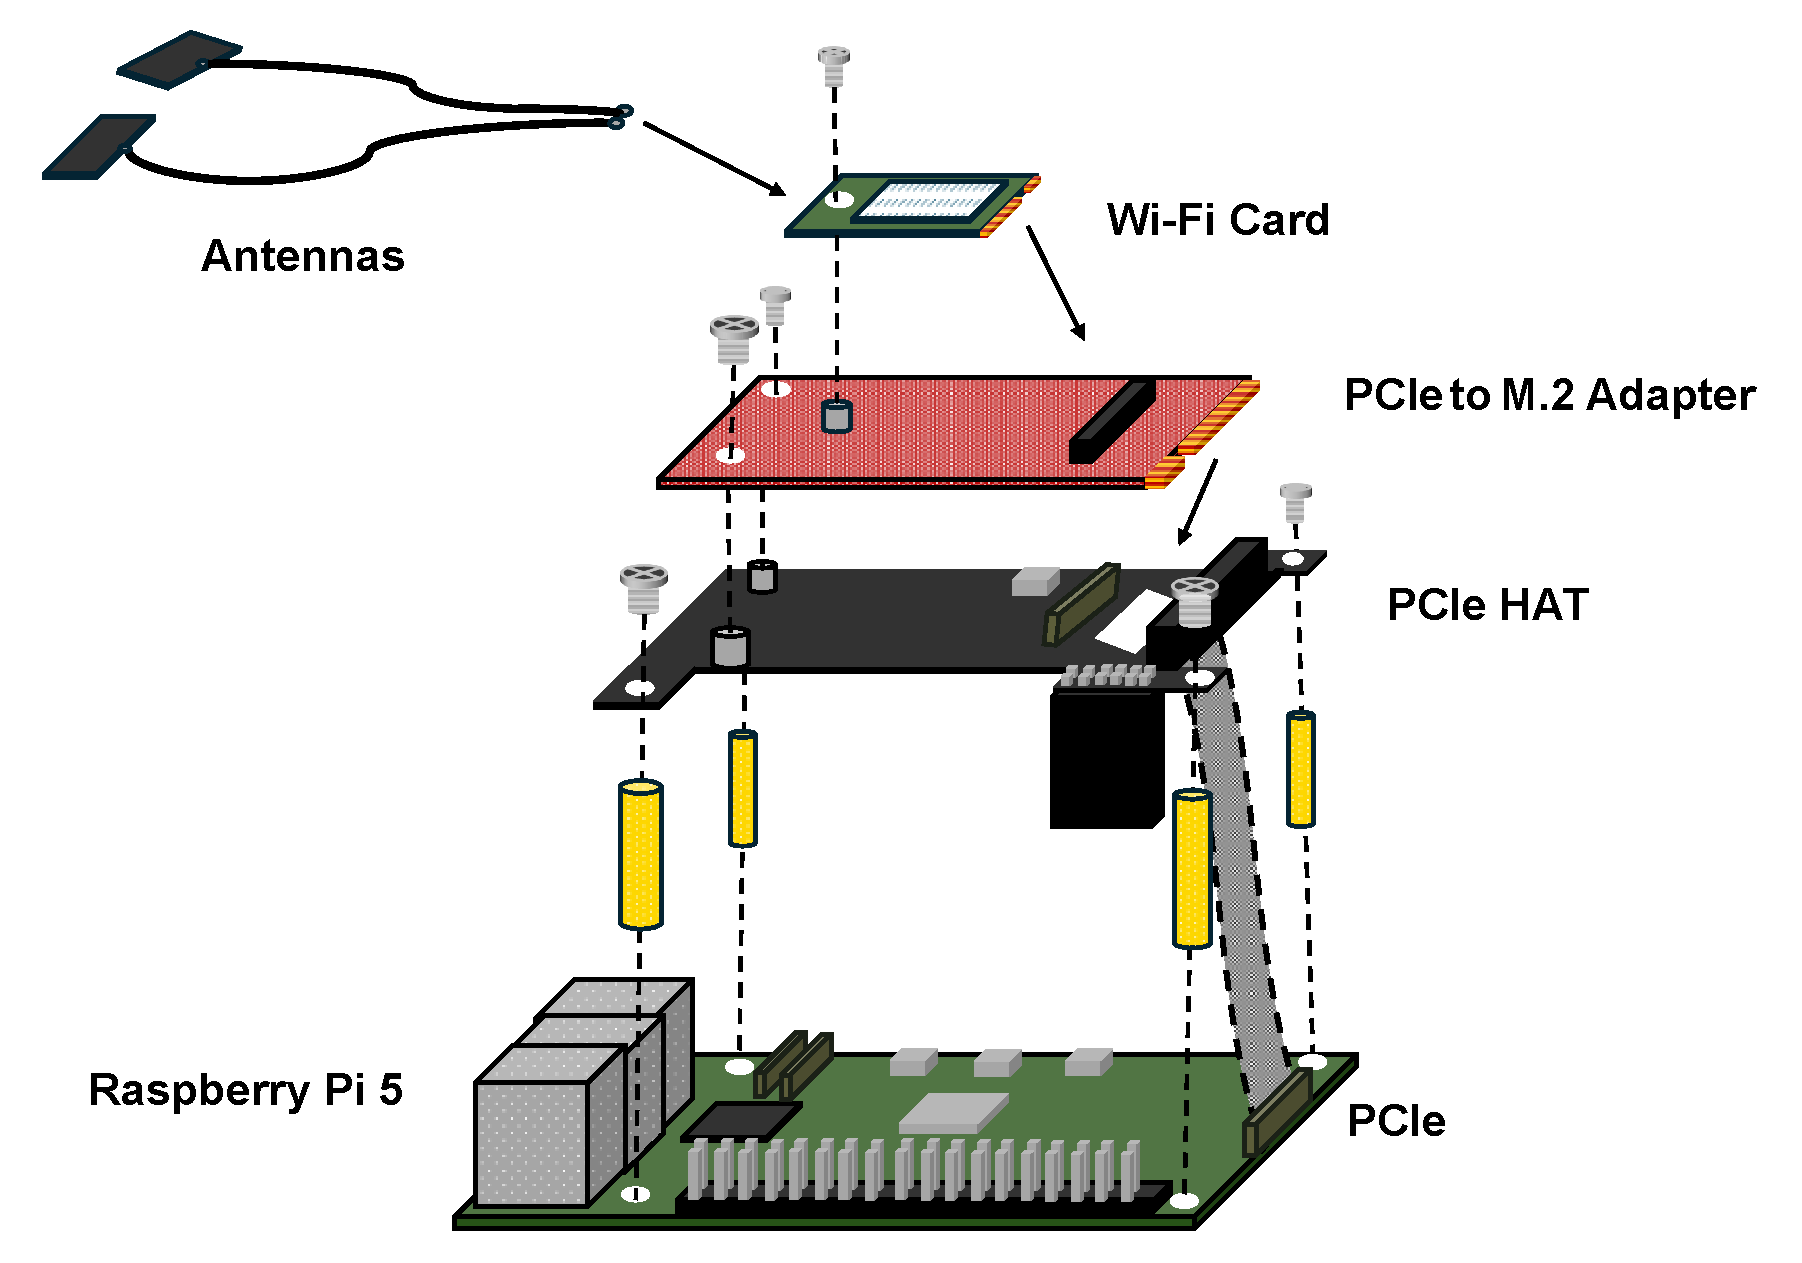
\includegraphics[width=0.8\linewidth]{figures/raspy.drawio.pdf}
    \caption{Presentation of the used hardware}
    \label{fig:hardware}
\end{figure}

Figure \ref{fig:hardware} shows the individual components of the hardware setup.  
As the computing unit, a Raspberry Pi 5B is used.  
This model is widely available and used.  
Earlier models, such as the Raspberry Pi 3, are, as described in \cite{raspy}, the third most sold computer of all time.  

For the Wi-Fi cards, the MT7925B22M from Mediatek was used.  
As stated in \cite{mt7925}, it supports Wi-Fi 7 and thus covers frequencies from 2.4 GHz to 6 GHz and Wi-Fi standards 4 through 6e.  
The card was released at the end of 2024, which is why the Wi-Fi 7 standard was not yet implemented in the driver at the time of this work, as indicated in \cite{mt76}.  
Nevertheless, the drivers are open source, although the firmware remains closed source.  
While changes are still being made to the driver, all standards up to Wi-Fi 6e can be used without errors.  

The most recent Wi-Fi cards with both open drivers and open firmware are those that use the ath9k driver, as shown in \cite{ath9k}.  
To include different drivers and firmware in the evaluation and to have access to fully open firmware, the AR5BXB92 from Qualcomm Atheros is used as additional card.  
This card was released in 2008 and only supports Wi-Fi 4 with 2.4 GHz and 5 GHz, as noted in \cite{ar5b}.  
Thus, it provides a strong contrast to the Mediatek card.  

As illustrated in Figure \ref{fig:hardware}, antennas must also be attached to the Wi-Fi cards.  
For the Mediatek card, a triband antenna is required, supporting 2.4 GHz, 5 GHz, and 6 GHz.  
For the Atheros card, a dual-band antenna is sufficient.  
Therefore, the ANT-W63-FPC2-ccc-100 \cite{te} is used for the Mediatek card, while the Molex 1461870050 \cite{molex} is used for the Atheros card.  

The Raspberry Pi 5 has a PCIe interface to which a PCIe HAT is attached, as shown in Figure \ref{fig:hardware}.  
This HAT provides a mini PCIe slot.  
For the Atheros card, this is sufficient, as it uses a mini PCIe connector.  
The Mediatek card, however, requires an M.2 Key E connector.  
Therefore, as also shown in Figure \ref{fig:hardware}, a mini PCIe to M.2 Key E adapter is installed.  
It must be ensured that the adapter supports M.2 Key E, since, as described in \cite[p. 24]{pcie}, Wi-Fi cards can use Key A, Key E, or Key A+E.  

Since this section has described the hardware used, the following section introduces the fundamentals of Yocto Linux.  
These are necessary to understand the configuration of the operating system, which is described in Chapter \ref{sec:os}.  

\section{Yocto Project} \label{subsec:yocto}
Das Yocto Project wurde 2010 von der Linux Foundation ins Leben gerufen, wie sie in \cite{The_Linux_Foundation_2011} berichtet.
Wie Salvador in Kapitel \cite[Chap. 1]{10251255} schreibt, ist das Yocto Projekt open source und in einem Zusammenschluss aus vielen Firmen, die das gemeinsame Ziel haben, Linux basierte eingebettete systeme zu bauen, entstanden.
Dabei war das primäre Ziel die duplicated Arbeit zu minimieren.

Das Yocto Project dient dazu eine Embedded Linux distribution zu bauen, wie Gonzales in \cite[Chap. 1]{Gonzalez_2018} beschreibt.
Dabei sollte diese so minimal wie möglich sein und modluar erweitert werden können.
Aus diesem Usecase leitet sich auch der Name des Projekts ab.
Wie in \cite[p. 29]{units} zu erkennen, ist Yocto eine sehr kleien Zahl, um genau zu sein $10^{-24}$.
Dies ist eine Metapher, dafür, dass mit dem Yocto Project eine sehr kleine Linux Distribution geabut werden kann.

Layer, Rezept, meta-openembedded
Phasen Rezept
\section{Linux Wi-Fi Stack} \label{subsec:linux_stack}
\section{Wi-Fi standards} \label{subsec:stand}
2,4 \cite[p. 2790]{9363693} 
\subsection{Quality of Service} \label{subsec:qos}
\subsection{IEEE 802.11n}
\subsection{IEEE 802.11ac}
\subsection{IEEE 802.11ax}
\subsection{IEEE 802.11be}
\section{Medium Access Mechanisms} \label{subsec:mac}
\section{Real Time} \label{sec:real_time}
In this chapter, the fundamentals of real-time systems are explained.  
First, Chapter \ref{subsec:rts} introduces the foundations of real-time capability and provides definitions of key terms.  
Afterwards, Chapter \ref{subsec:real_time_kernel} discusses how real-time capability can be ensured or improved in Linux.  

\subsection{Real Time Systems} \label{subsec:rts}
As Mächtel and Quade describe in \cite[Chap. 1]{Quade_Maechtel_2012}, the result of a real-time system depends not only on correctness but also on a temporal component.  
A real-time task has a time window in which the result must be delivered.  
Otherwise, the result loses its value.  
This time window is defined in Figure \ref{fig:utility} by a minimum threshold $T_{Dmin}$ and a maximum threshold $T_{Dmax}$.  
A good example is a pacemaker.  
It is not sufficient that the pacemaker is able to deliver an electric pulse, it must do so at the correct time.  
If the pulse is delivered too early or too late, the patient will most likely suffer harm rather than being stabilized.  

As Quade and Mächtel explain in \cite[p. 24]{Quade_Maechtel_2012}, different types of real-time systems are distinguished.  
Figure \ref{fig:utility} illustrates the three types soft, firm, and hard real-time systems.  
In a soft real-time system, shown in Figure \ref{subfig:soft}, the value of the result decreases the further it deviates from the deadlines.  
In a firm real-time system, shown in Figure \ref{subfig:firm}, the value of the result drops immediately to zero if the boundaries are violated.  
In a hard real-time system, as shown in Figure \ref{subfig:hard}, the value of the result even becomes negative as soon as the boundaries are violated.  
Strictly speaking, there are no negative percentages, but the figure illustrates that in hard real-time systems, failing to meet the deadline does not merely render the result useless, but even it may cause harm.  
This is the case, for example, with a pacemaker.  

\begin{figure}[h!]
    \centering
    \begin{subfigure}[b]{0.3\textwidth}
        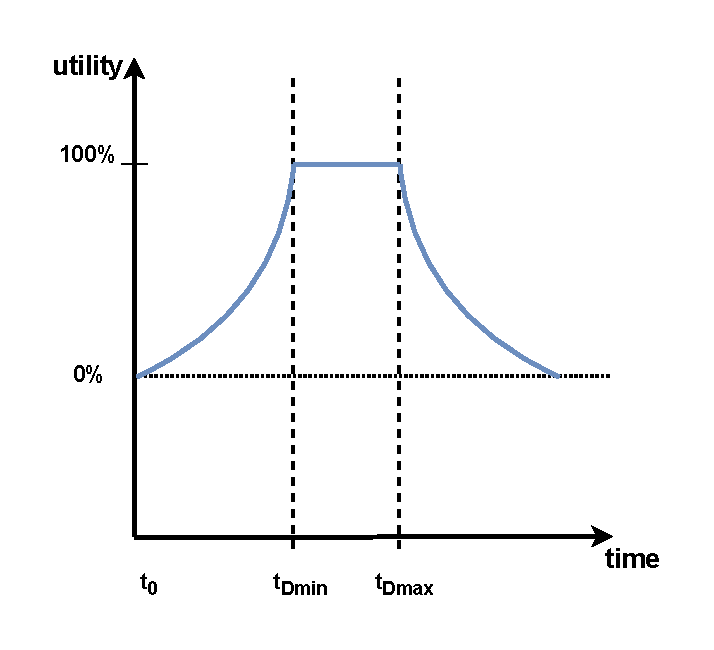
\includegraphics[width=\textwidth]{figures/real time.drawio.pdf}
        \caption{Presentation of the soft real time utility function}
        \label{subfig:soft}
    \end{subfigure}
    \hfill
    \begin{subfigure}[b]{0.3\textwidth}
        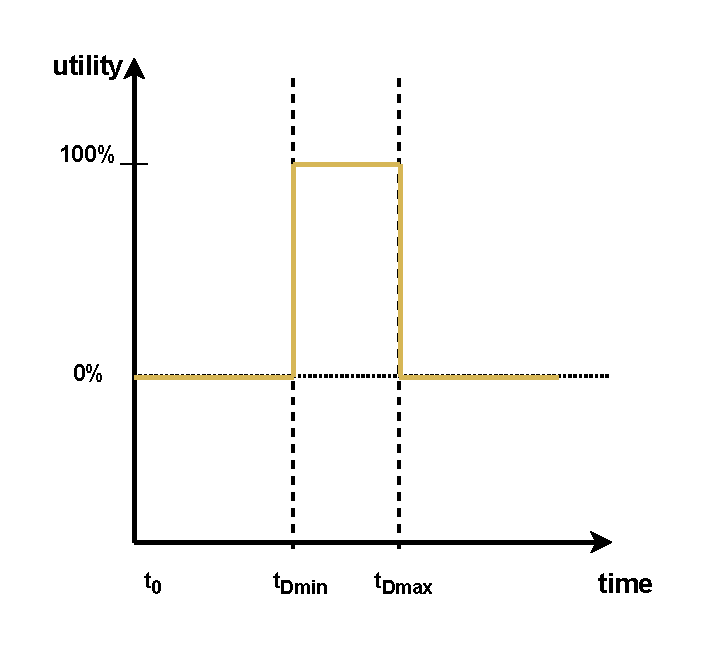
\includegraphics[width=\textwidth]{figures/firm-real-time.drawio.pdf}
        \caption{Presentation of the firm real time utility function}
         \label{subfig:firm}
    \end{subfigure}
    \hfill
    \begin{subfigure}[b]{0.3\textwidth}
        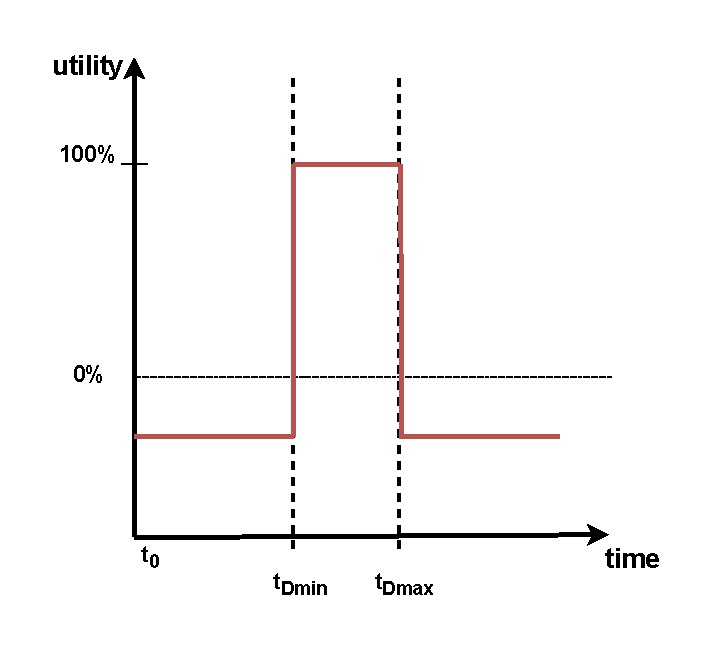
\includegraphics[width=\textwidth]{figures/hard-real-time.drawio.pdf}
        \caption{Presentation of the hard real time utility function}
         \label{subfig:hard}
    \end{subfigure}
    \caption{Presentation of the utility functions for soft, firm and hard real time}
     \label{fig:utility}
\end{figure}

To guarantee that a specific task delivers its result within these boundaries, both the task and the system must be fully predictable.  
This predictability is referred to as \textbf{determinism}.  
A task with real-time constraints usually occurs repeatedly, in other words, periodically.  
This does not necessarily mean in a fixed cycle.  
Thus, a minimum period $T_{Pmin}$ and a maximum period $T_{Pmax}$ exist, which separate two task executions.  

To ensure that a task always terminates within its real-time boundaries, this would ideally be proven mathematically.  
However, in systems with sporadic events this is difficult to achieve, which is why probabilistic approaches are often used.  
In other words, the \ac{WCET} of a task is determined, either mathematically or through repeated measurements.  
Using this, the maximum utilization $U_{max}$ can then be calculated.  
It is defined as $U_{max} = \frac{T_{WCET}}{T_{Pmin}}$, i.e. the longest execution time divided by the shortest distance between two events.  
If this value is below 1, the system should function correctly.  
According to Liu and Layland \cite[p. 9]{10.1145/321738.321743}, $U_{max}$ for many processes converges to $\ln(2)$, corresponding to $U_{max} = 0.69$.  
In practice, however, a more conservative threshold of $U_{max} < 0.5$ has proven effective, providing sufficient buffer.  
If a system is able to meet its real-time requirements, this property is referred to as \textbf{timeliness}.  

In addition to execution time and the number of deadline misses, jitter is frequently used as a quality metric for real-time systems, as described in \cite[p. 38]{real_time_systems}.  
Jitter refers to the temporal deviation from an expected event.  
For example, if the period $t$ is 3 ms and the start time is $t_0$, the following event is expected at $t_0 + 3$ ms.  
On a real system, however, it may occur at $t_0 + (3-x)$ ms, where $x \in [0, 3]$.  
This deviation $x$, i.e., the difference from the expected occurrence, is referred to as jitter and serves as a measure of the real-time capability of the system.  
The lower the jitter, the more deterministic the system is and thus the higher its real-time quality.  

The following section discusses how Linux can be made more real-time capable and which properties are most relevant in this regard.  

\subsection{Real Time Kernel} \label{subsec:real_time_kernel}
As described in Chapter \ref{subsec:yocto}, this work relies on Linux as the operating system.  
However, as noted in \cite{not_rt}, Linux does not inherently provide real-time capabilities.  
Additional functionalities not included in the standard Linux kernel can be introduced through extensions and modifications.
Theses are called patches.  
With the Preempt-RT patch, hereafter referred to as the RT-patch, Linux can be extended to meet the requirements of a real-time operating system\footnote{It is important to note that even with the RT-patch, Linux is not fully real-time capable, as demonstrated by a NASA study \cite{nasa}. Nevertheless, it is widely adopted in real-time applications, including by NASA and SpaceX, since it offers strong real-time capabilities while preserving the functionality of Linux.}.  

As discussed in Chapter \ref{subsec:rts}, a real-time system must be deterministic, i.e., predictable.  
It must be possible to determine the \ac{WCET} of a process and no spontaneous events may disrupt its execution.  

The RT-patch was initiated in 2005 by Steven Rostedt and others.  
As Rostedt explains in \cite{rt_patch}, one of the main causes of such unpredictable interruptions are hardware-generated interrupts.  
These signals, used by devices to communicate with the \ac{CPU}, are handled in \acp{ISR}.  
In conventional Linux systems, \acp{ISR} preempt processes, preventing the reliable determination of \ac{WCET}.  

In Linux, including with the RT-patch, processes are scheduled based on priority.  
Priorities range from $-100$ to $39$, whereas the lower number is the higher priority.  
For non-real-time processes, the priority $P$ is calculated as $P = 20 + NV$, where $NV$ is the nice value in the range $[-20, 19]$.
The default of the niche value is $0$.  
Thus, normal processes have priorities in the range $[0, 39]$.  
For real-time processes, $P = -1 - rt\_Prior$, where $rt\_Prior$ ranges from $[0, 99]$  yielding a priority range of $[-100, -1]$.  
As before $rt\_Prior$ has a default value of $0$.
Consequently, real-time processes are always preferred over non-real-time processes.  
Depending on the model of priorites they have different ranges.
In Linux the priorities often have a range of $[0, 139]$, where $139$ the highest priority is.
But for calculation of the priorities the model described before is used.

Interrupt handling is also adapted by the RT-patch.  
As described in \cite[p. 162]{rt_patch}, almost all\footnote{Exceptions exist, as noted in \cite[p. 163]{rt_patch}. Essential interrupts such as the timer interrupt are not threaded.} \acp{ISR} are moved into kernel threads.  
A distinction is made between hard \acp{IRQ} and soft \acp{IRQ}.  
Both are threaded, but while hard \acp{IRQ} remain non-preemptible, their execution becomes schedulable once threaded.  
Soft \acp{IRQ}, in contrast, are both schedulable and preemptible.  

Furthermore, the RT-patch introduces full kernel preemption.  
This means that user processes with sufficiently high priority can preempt kernel activities.  
Additionally, spinlocks and other blocking mechanisms have been replaced by mutexes to mitigate issues such as deadlocks and priority inversion.  
These modifications significantly improve the determinism of Linux under the RT-patch.  

This chapter has outlined the key concepts relevant for this thesis.  
The following section reviews related work and situates the objectives of this study within the broader research context.  
